\documentclass[12pt, twocolumn]{article}

% 引入相关的包
\usepackage{amsmath, listings, fontspec, geometry, graphicx, ctex, color, subfigure}

% 设定页面的尺寸和比例
\geometry{left = 1.5cm, right = 1.5cm, top = 1.5cm, bottom = 1.5cm}

% 设定两栏之间的间距
\setlength\columnsep{1cm}

% 设定字体,为代码的插入作准备
\newfontfamily\ubuntu{Ubuntu Mono}

% 头部信息
\title{\normf{这是标题}}
\author{\normf{陈烁龙}}
\date{\normf{\today}}

% 代码块的风格设定
\lstset{
	language=C++,
	basicstyle=\scriptsize\ubuntu,
	keywordstyle=\textbf,
	stringstyle=\itshape,
	commentstyle=\itshape,
	numberstyle=\scriptsize\ubuntu,
	showstringspaces=false,
	numbers=left,
	numbersep=8pt,
	tabsize=2,
	frame=single,
	framerule=1pt,
	columns=fullflexible,
	breaklines,
	frame=shadowbox, 
	backgroundcolor=\color[rgb]{0.97,0.97,0.97}
}

% 字体族的定义
\newcommand{\normf}{\kaishu}
\newcommand{\boldf}{\heiti}
\newcommand\keywords[1]{\boldf{关键词:} \normf #1}

\begin{document}
	
	% 插入头部信息
	\maketitle
	% 换页
	\thispagestyle{empty}
	\clearpage
	
	% 插入目录、图、表并换页
	\tableofcontents
	\listoffigures
	\listoftables
	\setcounter{page}{1}
	% 罗马字母形式的页码
	\pagenumbering{roman}
	\clearpage
	% 从该页开始计数
	\setcounter{page}{1}
	% 阿拉伯数字形式的页码
	\pagenumbering{arabic}
	
	\section{\normf{概述}}
	\normf
	本次论文为:《Targetless Calibration of LiDAR-IMU System Based on Continuous-time Batch Estimation》,其是一篇关于传感器标定的文章。其使用B样条曲线,在连续时间上对传感器的轨迹进行建模(主要是IMU和激光雷达)。其不需要靶标,适应的场景较多。
	
	\section{\normf{前置知识}}
	\subsection{\normf{贝塞尔曲线}}
	贝塞尔曲线主要用于二维图形应用程序中的数学曲线,曲线由起始点,终止点(也称锚点)和控制点组成,通过调整控制点,通过一定方式绘制的贝塞尔曲线形状会发生变化(注意是整体曲线,这和后面的B样条曲线不同)。
	
	对于$n$次的贝塞尔曲线,其有$n+1$个控制点,曲线上点的位置由控制点和参数$t\in[0,1]$决定。其公式为:
	\begin{equation*}
		B_n(t)=\sum_{i=0}^{n}C_{n}^{i}(1-t)^{n-i}t^{i}P_{i}\quad t\in[0,1]
	\end{equation*}
	其中:
	\begin{equation*}
		C_{n}^{i}=\frac{n!}{(n-i)!\cdot i!}
	\end{equation*}
	例如,对于3阶的贝塞尔曲线,其公式为:
	\begin{equation*}
		\begin{aligned}
			B_3(t)=&(1-t)^3P_0+3t(1-t)^2P_1\\&+3t^2(1-t)P_2+t^3P_3
		\end{aligned}
	\end{equation*}
另外,对于计算机适合的计算贝塞尔曲线递推方法为:
\begin{equation*}
	\begin{aligned}
			&B_n(t|P_0,P_1,\dots,P_n)=\\&(1-t)B_{n-1}(t|P_0,P_1,\dots,P_{n-1})\\
			&+tB_{n-1}(t|P,P_1,\dots,P_n)
	\end{aligned}
\end{equation*}
比如,同样对于3阶的贝塞尔曲线,其公式为:
\begin{equation*}
	\begin{cases}
		\begin{aligned}
			B_3(t|P_0,P_1,P_2,P_3)=&(1-t)B_2(t|P_0,P_1,P_2)\\&+tB_2(t|P_1,P_2,P_3)
		\end{aligned}\\
		\begin{aligned}
		B_2(t|P_0,P_1,P_2)=&(1-t)B_1(t|P_0,P_1)\\&+tB_1(t|P_1,P_2)
		\end{aligned}\\
	\begin{aligned}
	B_2(t|P_1,P_2,P_3)=&(1-t)B_1(t|P_1,P_2)\\&+tB_1(t|P_2,P_3)
	\end{aligned}\\
	\begin{aligned}
	B_1(t|P_i,P_j)=&(1-t)B_0(t|P_i)+tB_0(t|P_j)\\
	=&(1-t)P_i+tP_j
	\end{aligned}
	\end{cases}
\end{equation*}
贝塞尔曲线如下图所示:
\begin{figure}[htbp]
	\centering
	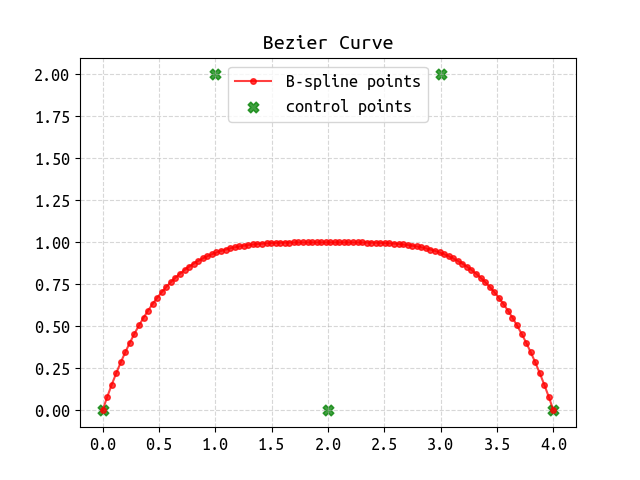
\includegraphics[width=0.9\linewidth]{../img/bezier.png}
	\caption{\normf{贝塞尔曲线}}
\end{figure}

	\subsection{\normf{B样条曲线}}
	B样条是通过一组指定点集而生成平滑曲线的柔性带。简单地说,B样条曲线就是通过控制点局部控制形状的曲线(注意是局部控制)。
	
	对于$m$阶$n$次B样条曲线($2\le n \le m+1$),其有$m+1$个节点分布在$[0,1]$,即:$0\le t_0<\dots<t_m\le 1$。其公式为:
	\begin{equation*}
		B_m(t)=\sum_{i=0}^{m}P_i\cdot b_{i,n}(t)\quad t\in[0,1]
	\end{equation*}
	其中$b_{i,n}(t)$可以通过Cox-de Boor递归公式得到:
	\begin{equation*}
		\begin{aligned}
			b_{i,n}&=\begin{cases}
				1\quad t_i<t<t_{i+1}\\
				0\quad\dots
			\end{cases}\\
		b_{i,n}&=\frac{t-t_i}{t_{i+n}-t_i}b_{i,n-1}(t)+\frac{t_{i+n+1}-t}{t_{i+n+1}-t_{i+1}}b_{i+1,n-1}(t)
		\end{aligned}
	\end{equation*}
	当节点等距,称B样条为均匀。
	
	
	
	
	
	
	
	
	
	
	
	
	
\end{document}

